\documentclass{article}
\usepackage{graphicx} % Required for inserting images
\usepackage{pdflscape}
\usepackage[margin=1in]{geometry}
\usepackage{fancyhdr}
\usepackage{listings}
\usepackage{courier}
\usepackage{multicol}
\usepackage{anyfontsize}
\usepackage{tcolorbox} % Required for the border around the entire document

% Header and Footer
\pagestyle{fancy}
\fancyhf{}
\fancyhead[RO,LE]{\textbf{Escuela de código PILARES}}
\fancyfoot[LO,CE]{Carlos Ignacio Padilla Herrera}
\fancyfoot[RO,RE]{\thepage}

% Listings settings
\lstset{
    basicstyle=\fontsize{8}{11}\selectfont\ttfamily,
    breaklines=true,
    captionpos=b,
    numbers=left,
    numberstyle=\tiny,
    stepnumber=1,
    numbersep=5pt,
    showspaces=false,
    showstringspaces=false,
    showtabs=false,
    tabsize=2,
    columns=fullflexible,
    frame=single, % Add a frame around the code
}

% Title Page
\title{02. Variables}
\author{Carlos Ignacio Padilla Herrera}
\date{03 de junio de 2024}

\begin{document}

% Add a border around the entire document
\tcbset{
    colframe=black, % Frame color
    colback=white, % Background color
    width=\textwidth, % Box width
    enlarge left by=\dimexpr\hoffset+\oddsidemargin+1in\relax,
    enlarge right by=\dimexpr\hoffset+\oddsidemargin+1in\relax,
    top=0pt, bottom=0pt, left=0pt, right=0pt, % Margins inside the box
    boxrule=1pt, % Border thickness
}

\tcbstartrecording

% Cover Page
\begin{titlepage}
    \centering
    \vspace*{2cm}

    \Huge
    \textbf{02. Variables}

    \vspace{1.5cm}

    \LARGE
    \textbf{Padilla Herrera Carlos Ignacio}

    \vspace{0.5cm}

    \Large
    \textbf{Folio: 794DR02}

    \vspace{1.5cm}

    \LARGE
    \textbf{Escuela de Código PILARES}


    \LARGE
    \textbf{Java Entre Semana G0224}

    \vspace{0.5cm}

    \Large
    Fecha: 03 de junio de 2024

    \vfill
\end{titlepage}

\maketitle

\section*{02. Variables}
\textbf{Objetivo:} Verificar el dominio teórico y técnico de los principios básicos de java mediante preguntas de opción múltiple y ejercicios para desarrollar su código.

\textbf{Indicaciones:} Realiza los programas que se te solicitan, una vez realizado sube el archivo de tu actividad.

\section*{Actividades}

\subsection*{Programa 1. (2 puntos)}
Crea un programa llamado \textbf{Booleans.java} que contenga lo siguiente:

\begin{itemize}
    \item Crea una variable llamada \textit{intsPuedeAlmacenarDecimales}. Ponlo en verdadero (True) si el tipo \textit{int} puede contener un número decimal. Ponlo en falso (false) si el tipo \textit{int} no puede hacer esto.
    \item Imprime la variable \textit{intsPuedeAlmacenarDecimales}.
    \item Escribe la salida del programa.
    \item Toma captura de pantalla del código completo y del programa compilado.
\end{itemize}

\begin{lstlisting}[language=Java, caption={Código del programa Booleans.java}]
/*
 * Click nbfs://nbhost/SystemFileSystem/Templates/Licenses/license-default.txt to change this license
 */

package com.mycompany.booleans;

/**
 *
 * @author enigma
 */
public class Booleans {

    public static void main(String[] args) {
        boolean intsPuedeAlmacenarDecimales = false;
        System.out.println("El tipo int puede almacenar decimales? " + intsPuedeAlmacenarDecimales);
    }
}
\end{lstlisting}

\newpage

\subsection*{Programa 2. (2 puntos)}
Crea un programa llamado \textbf{Char.java} que contenga lo siguiente:

\begin{itemize}
    \item Escribe como comentario de una sola línea tu nombre.
    \item Crea una variable llamada \textit{primerLetra} de tipo \textit{char} y almacena ahí la primera letra de tu nombre.
    \item Imprime en la terminal el valor de la variable \textit{primerLetra}.
    \item Escribe la salida.
    \item Toma captura de pantalla del código completo y del programa compilado.
\end{itemize}

\begin{lstlisting}[language=Java, caption={Código del programa Caracter.java}]
    /*
 * Click nbfs://nbhost/SystemFileSystem/Templates/Licenses/license-default.txt to change this license
 */

package com.mycompany.caracter;

/**
 *
 * @author enigma
 */
public class Caracter {

    public static void main(String[] args) {
        char primerLetra = 'C'; // Nombre Carlos
        System.out.println("La primera letra de mi nombre es: " + primerLetra);
    }
}

\end{lstlisting}
\newpage

\subsection*{Programa 3. (2 puntos)}
Crea un programa llamado \textbf{Poema.java} que contenga lo siguiente:

\begin{itemize}
    \item Crea una variable llamada \textit{verso} de tipo \textit{String} y almacena ahí el verso “Aquí no suceden cosas de mayor trascendencia que las rosas.”
    \item Invoca \textit{System.out.println()} para imprimir el valor de la variable \textit{verso}.
    \item Escribe la salida.
    \item Toma captura de pantalla del código completo y del programa compilado.
\end{itemize}

\begin{lstlisting}[language=Java, caption={Código del programa Poema.java}]
    /*
 * Click nbfs://nbhost/SystemFileSystem/Templates/Licenses/license-default.txt to change this license
 */

package com.mycompany.poema;

/**
 *
 * @author enigma
 */
public class Poema {

    public static void main(String[] args) {
        String verso = "Aqui no suceden cosas de mayor trascendencia que las rosas. ";
        System.out.println(verso);
    }
}

\end{lstlisting}


\newpage

\subsection*{Programa 4. (2 puntos)}
Crea un programa llamado \textbf{MiPerfil.java} que contenga lo siguiente:

\begin{itemize}
    \item El archivo \textit{MiPerfil.java} contiene una clase que representa tu perfil de contratación que se presentará a potenciales empleadores.
    \item En el método \textit{main()}, crea una variable llamada \textit{nombre} que contenga tu nombre, como una secuencia de caracteres.
    \item Crea una variable llamada \textit{edad} que contenga tu edad como un número entero.
    \item Crea una variable llamada \textit{salarioDeseado} que contenga tu salario deseado por mes con una precisión de dos puntos decimales.
    \item Crea una variable llamada \textit{genero} que contenga un solo carácter, m (masculino), f (femenino), n (para ninguno) u o (para otro).
    \item Crea una variable llamada \textit{buscandoTrabajo} que contenga si actualmente estás abierto a ofertas de trabajo o no.
    \item Imprime el valor de cada una de las variables, una por cada línea.
    \item Escribe la salida.
    \item Toma captura de pantalla del código completo y del programa compilado.
\end{itemize}

\begin{lstlisting} [language=Java, caption={Código del programa MiPerfil.java}]
    /*
 * Click nbfs://nbhost/SystemFileSystem/Templates/Licenses/license-default.txt to change this license
 */

package com.mycompany.miperfil;

/**
 *
 * @author enigma
 */
public class MiPerfil {

    public static void main(String[] args) {
        String nombre = "Carlos I. Padilla Herrera";
        int edad = 30;
        double salarioDeseado = 23000;
        char genero = 'm';
        boolean buscandoTrabajo = true;

        System.out.println("Nombre: " + nombre);
        System.out.println("Edad: " + edad);
        System.out.println("Salario Deseado: " + salarioDeseado);
        System.out.println("Genero: " + genero);
        System.out.println("Buscando Trabajo: " + (buscandoTrabajo ? "Si" : "No"));
    }
}

\end{lstlisting}

\newpage

\begin{landscape}
    \begin{figure}[h]
        \centering
        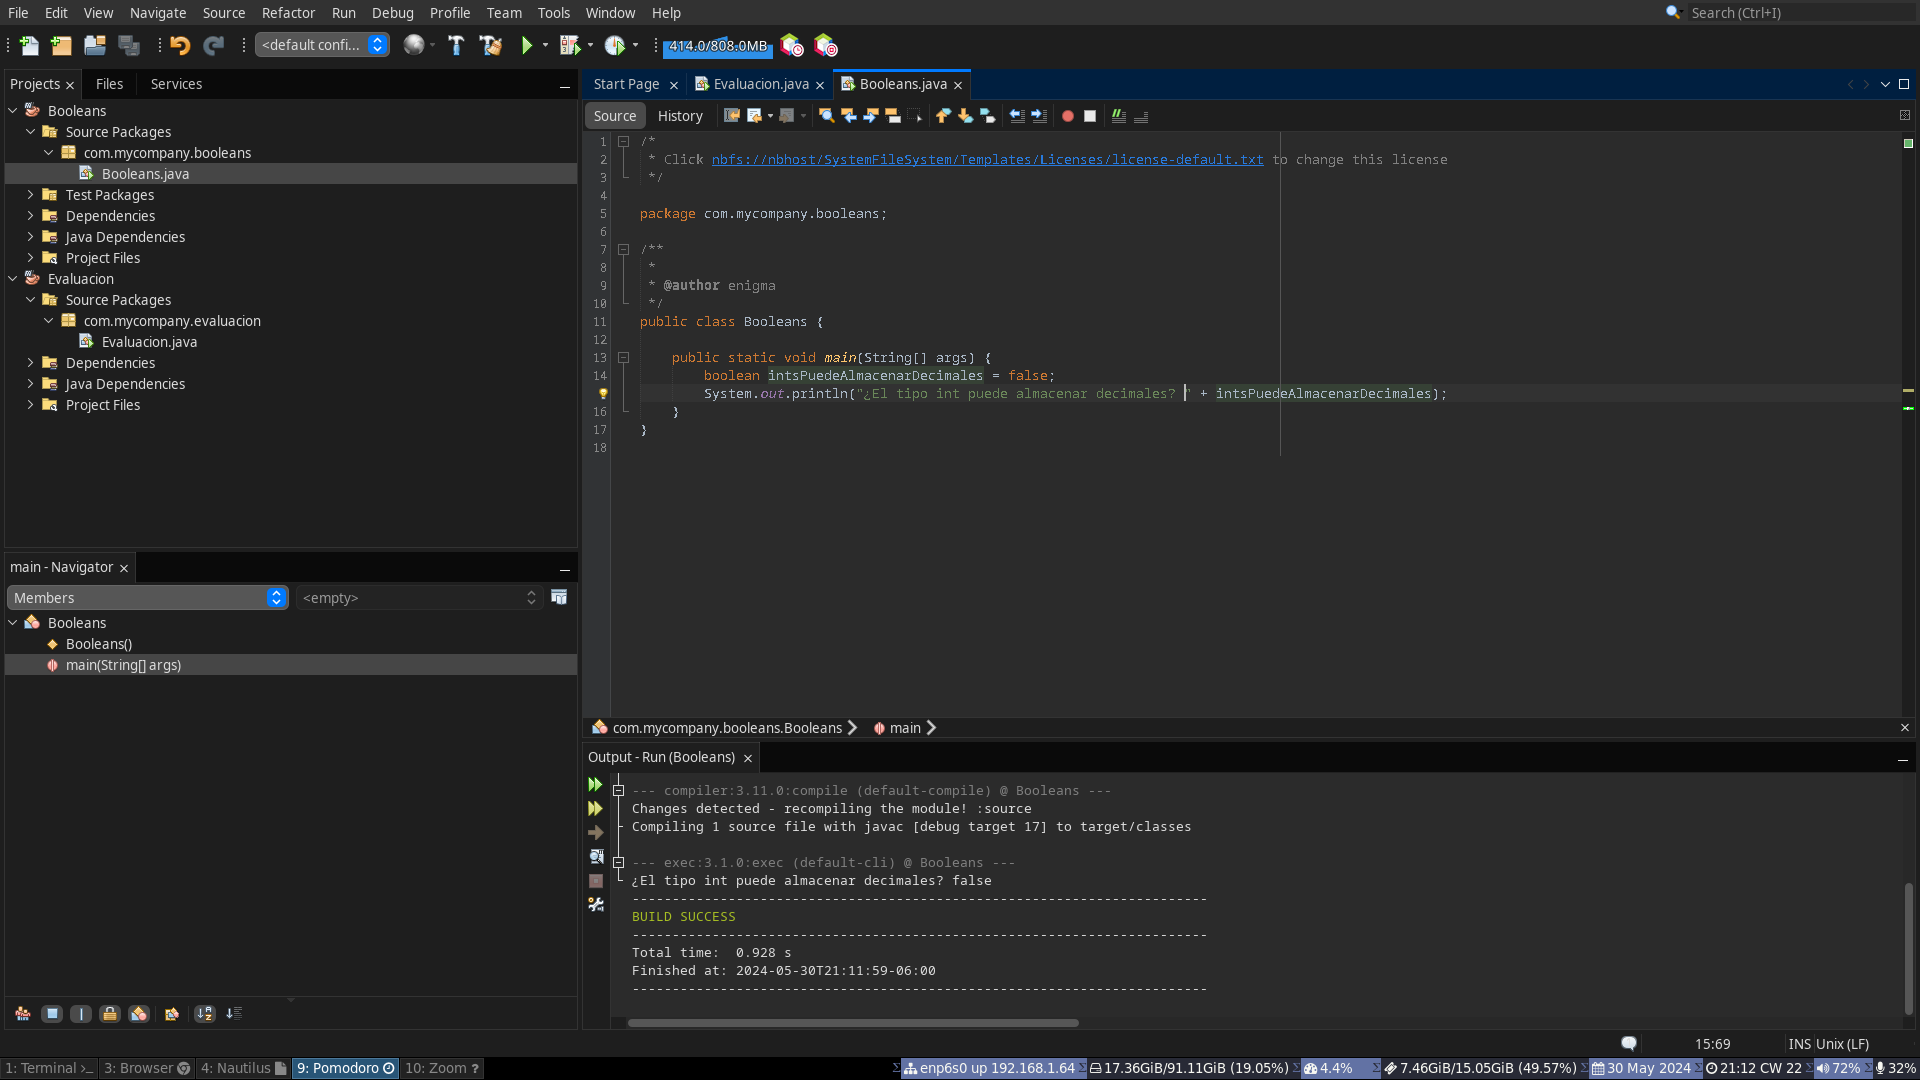
\includegraphics[width=\linewidth]{img/booleans.png}
        \caption{Captura del programa Booleans.java}
        \label{fig:captura}
    \end{figure}

    \newpage

    \begin{figure}[h]
        \centering
        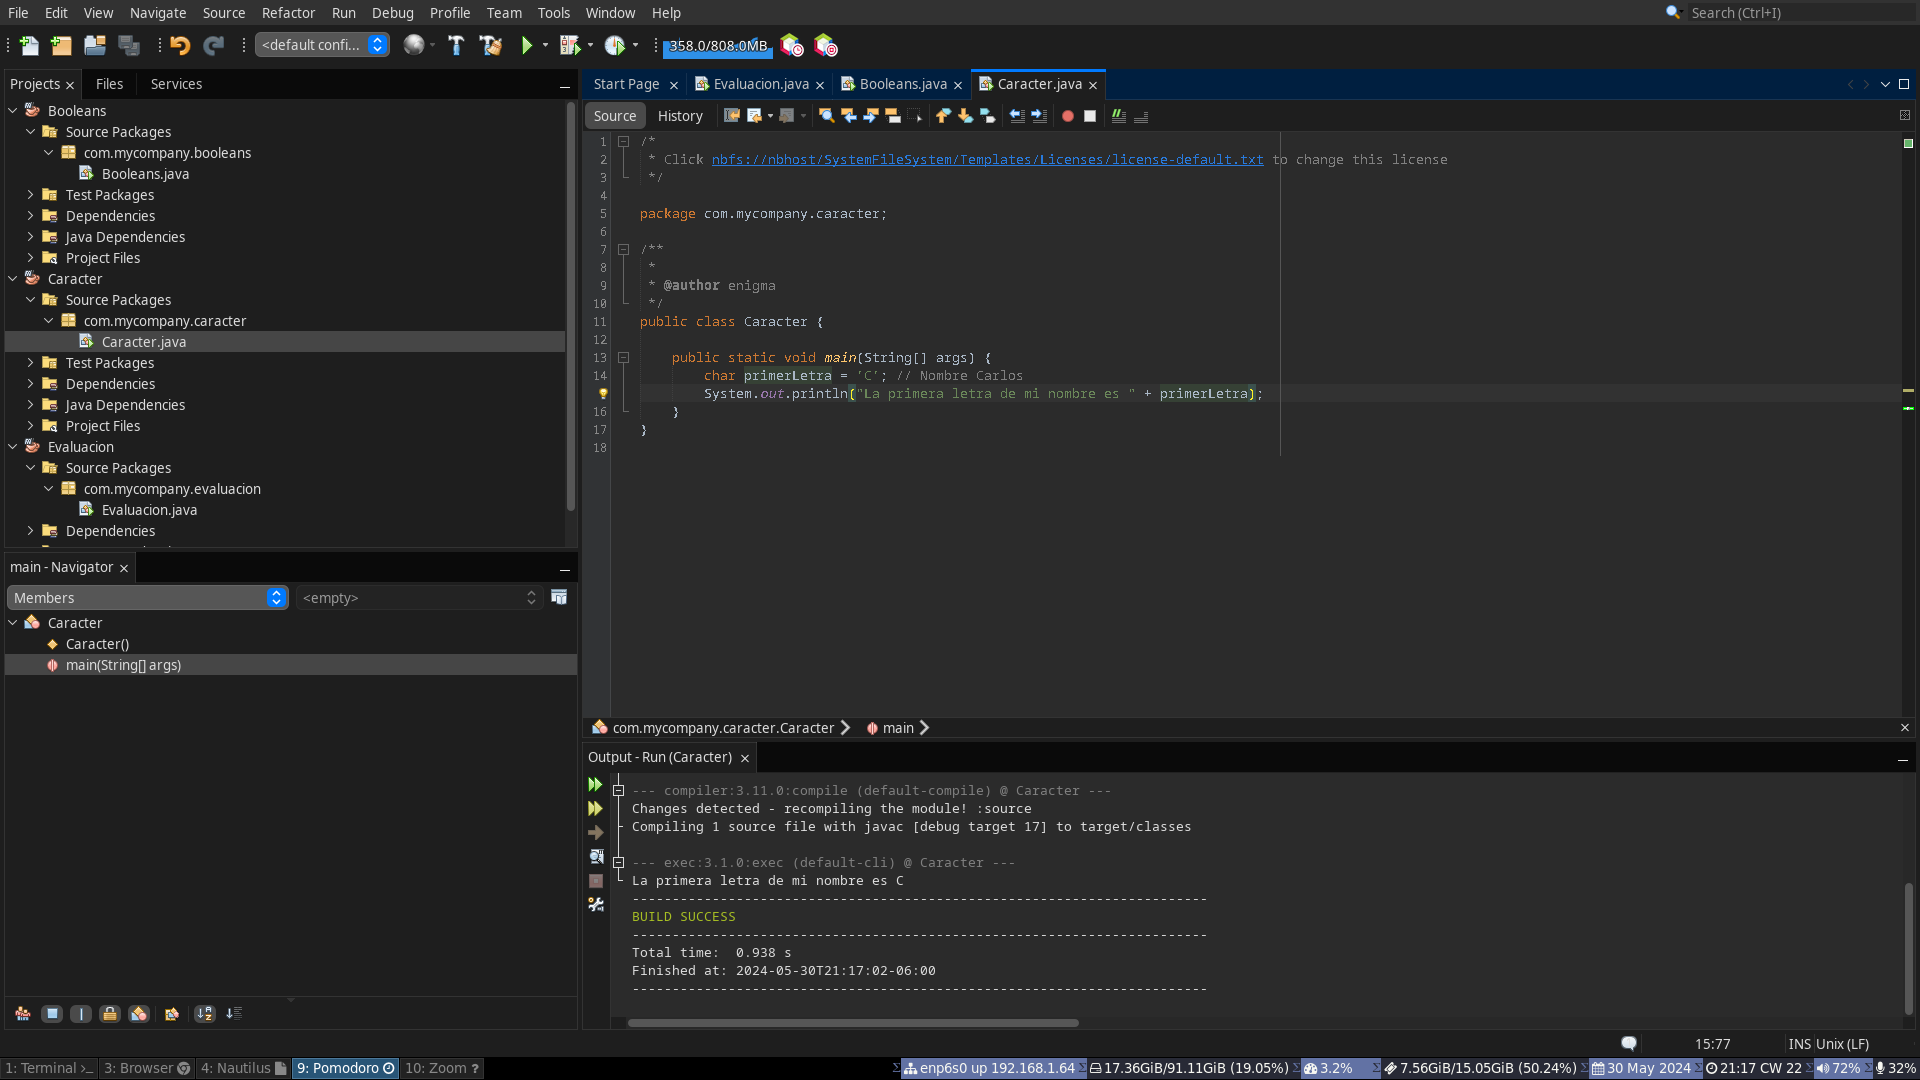
\includegraphics[width=\linewidth]{img/character.png}
        \caption{Captura del programa Char.java}
        \label{fig:captura}
    \end{figure}

    \newpage

    \begin{figure}[h]
        \centering
        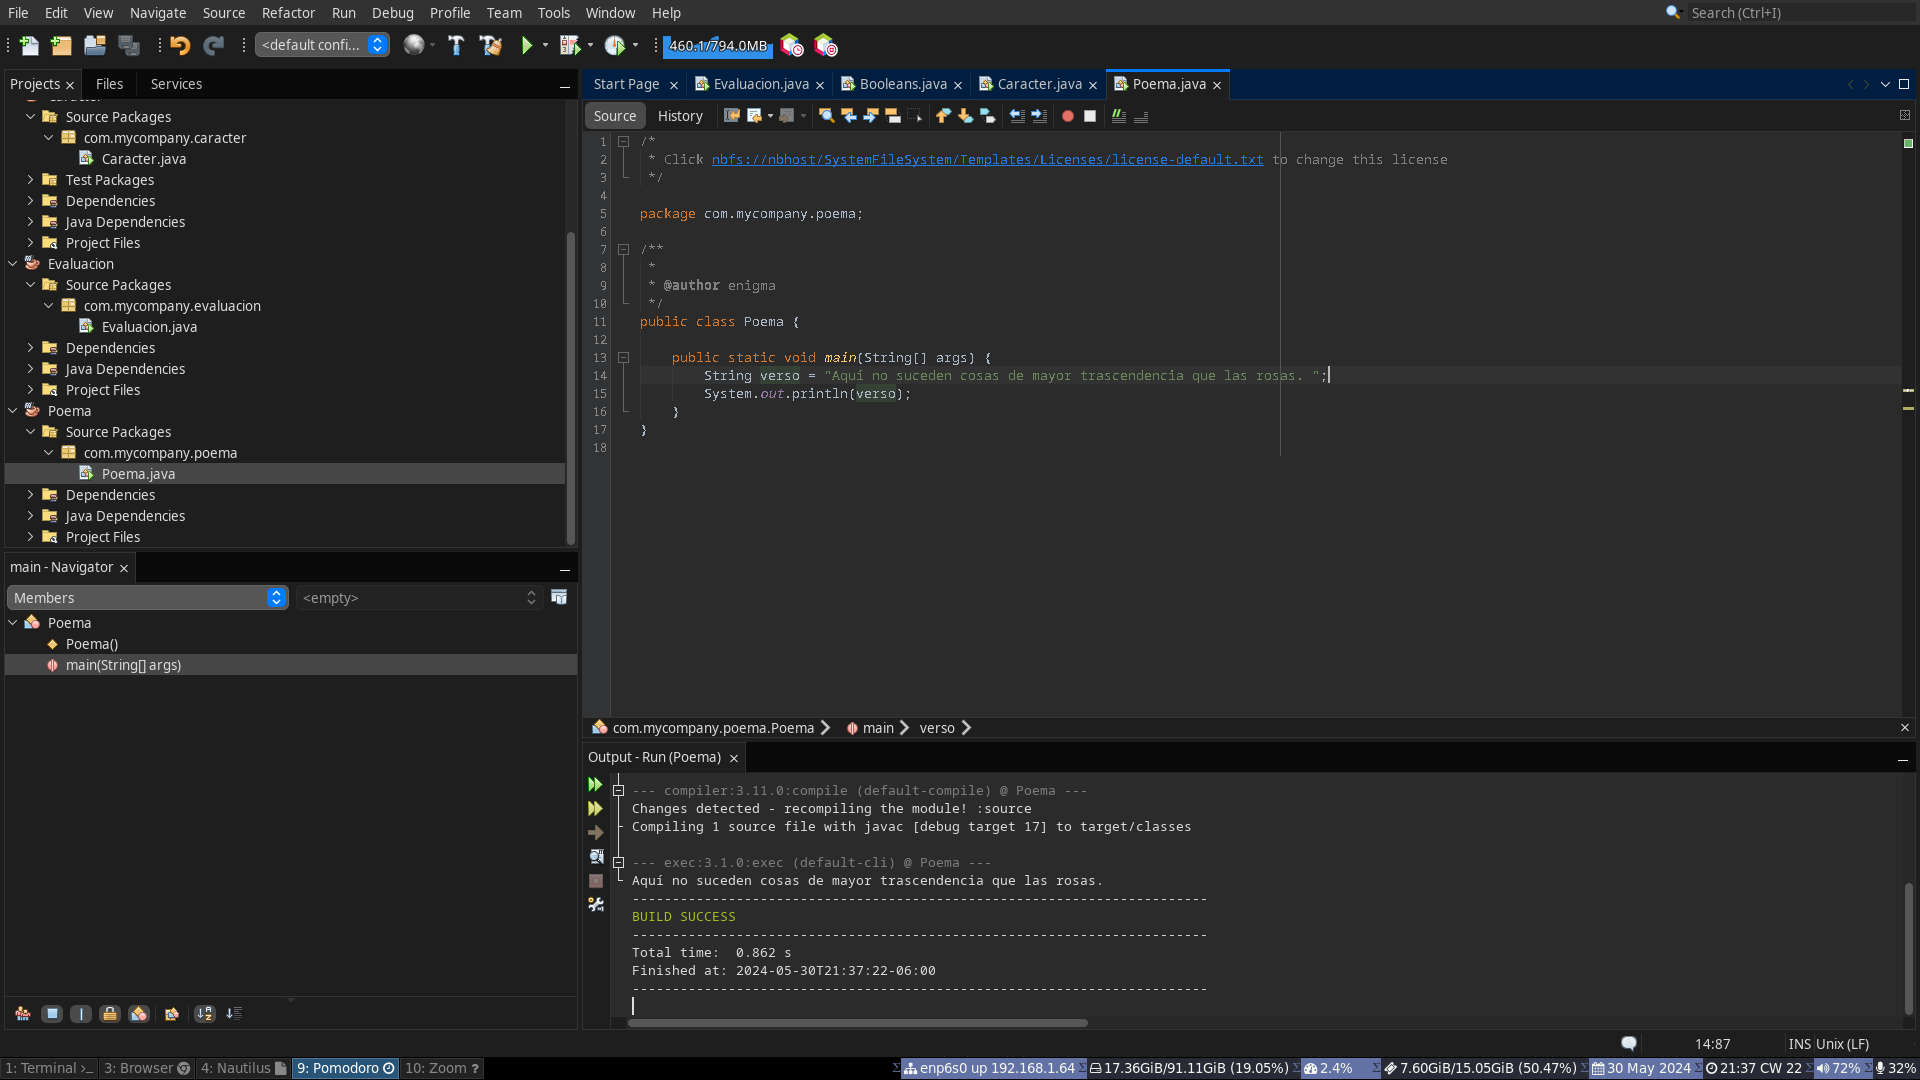
\includegraphics[width=\linewidth]{img/poema.png}
        \caption{Captura del programa Poema.java}
        \label{fig:captura}
    \end{figure}

    \newpage

    \begin{figure}[h]
        \centering
        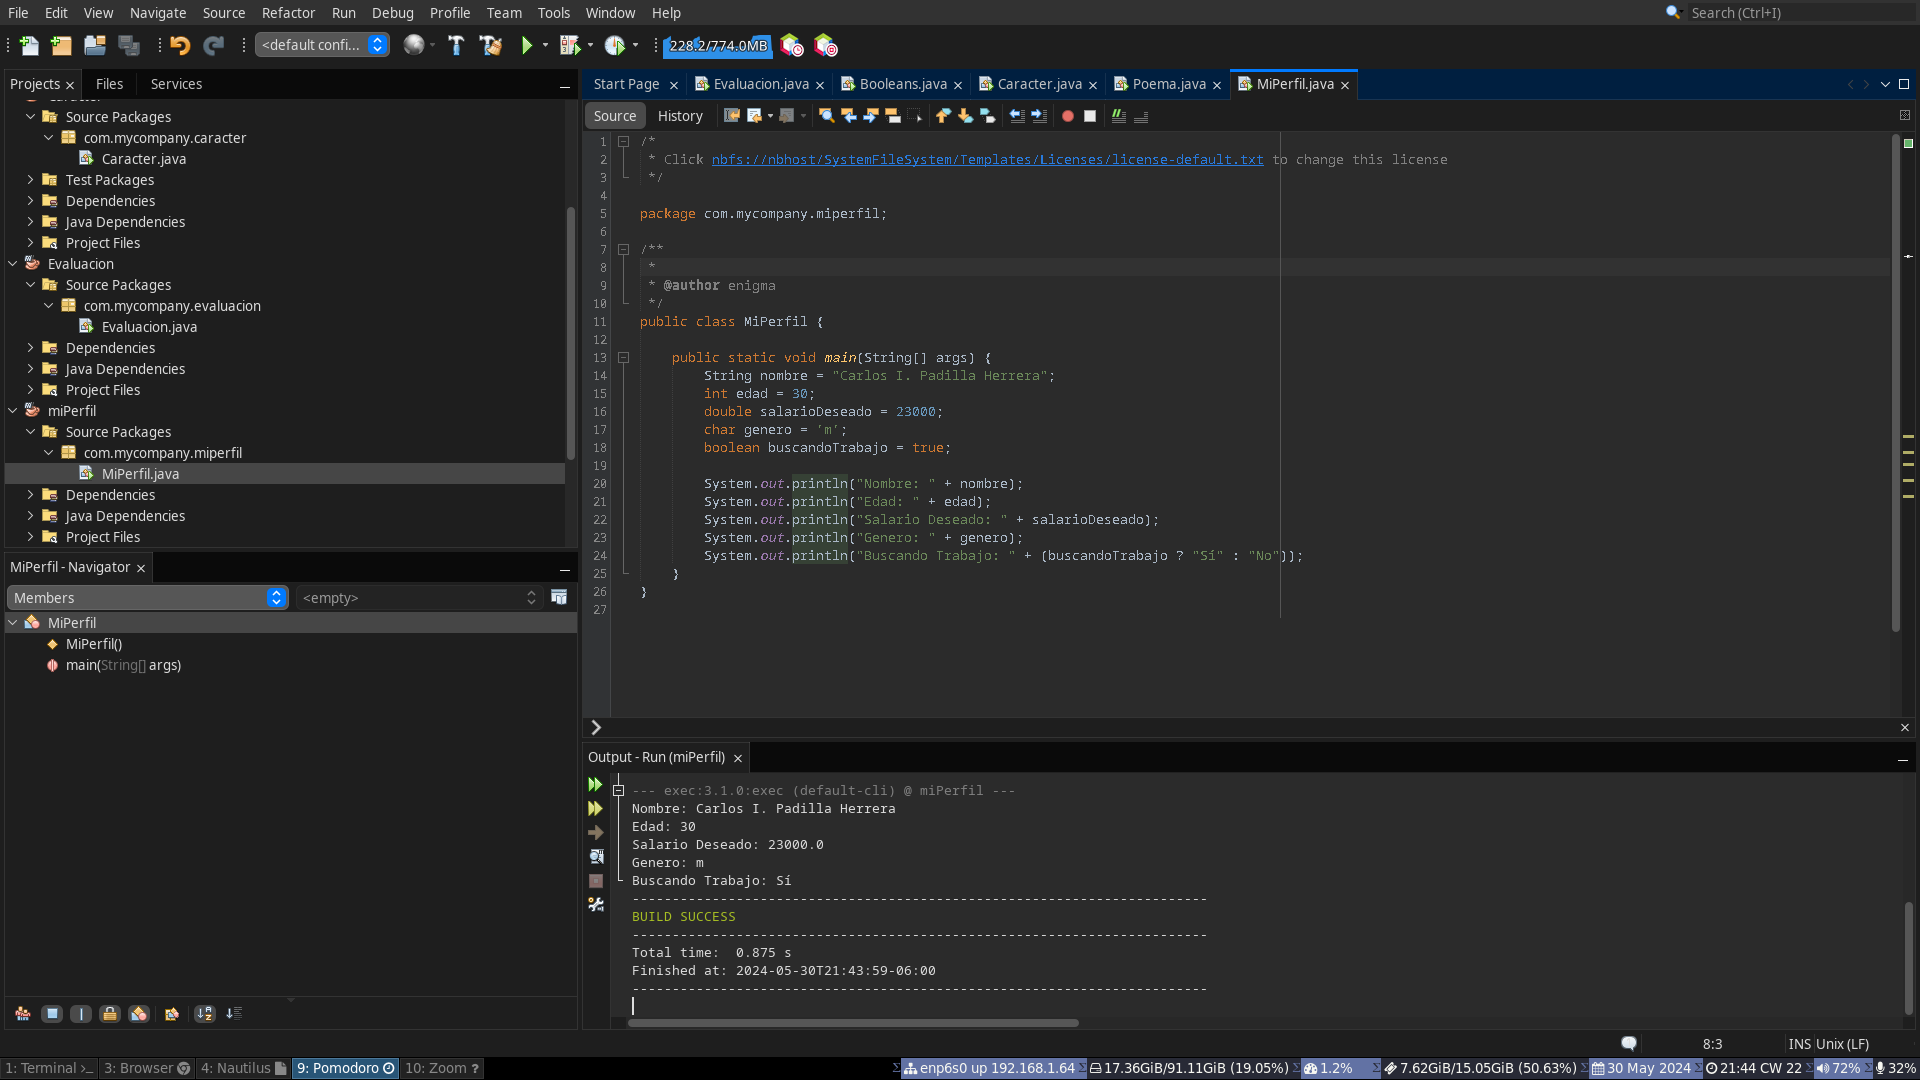
\includegraphics[width=\linewidth]{img/miPerfil.png}
        \caption{Captura del programa MiPerfil.java}
        \label{fig:captura}
    \end{figure}
\end{landscape}

\end{document}

\tcbset{record}
